%Metroplolis Beamer Theme: https://github.com/matze/mtheme
\documentclass[aspectratio=169, 10pt, dvipsnames]{beamer}
\usetheme{metropolis}
\usepackage{appendixnumberbeamer, lmodern, bookmark, kbordermatrix,fontawesome}
\usepackage{booktabs}
% \usepackage[sorting=none]{biblatex}
\usepackage[scale=2]{ccicons}
\usepackage{pgfplots}
\usepgfplotslibrary{dateplot}
\usepackage{xspace}
\newcommand{\themename}{\textbf{\textsc{metropolis}}\xspace}
\usepackage{bbm}
\usepackage{tikz, graphicx}
\usepackage{caption, subcaption}
\usepackage{multicol}
% \usepackage[dvipsnames]{xcolor}
\usepackage{scalerel,xparse}
\NewDocumentCommand\brain{}{
    \scalerel*{
        \includegraphics{/home/pjh/.emojis/u1F9E0.png}
    }{X}
  }
  \NewDocumentCommand\doughnut{}{
    \scalerel*{
        \includegraphics{/home/pjh/.emojis/u1F369.png}
    }{X}
  }
  \NewDocumentCommand\compass{}{
    \scalerel*{
        \includegraphics{/home/pjh/.emojis/u1F9ED.png}
    }{X}
  }
  \NewDocumentCommand\mug{}{
    \scalerel*{
        \includegraphics{/home/pjh/.emojis/u2615.png}
    }{X}
  }


\usetikzlibrary{shapes,arrows}
\tikzstyle{orange} = [rectangle, draw, fill=YellowOrange!30,
    text width=7em, text centered, rounded corners]
\tikzstyle{orange} = [rectangle, draw, fill=YellowOrange!30,
    text width=7em, text centered, rounded corners]
\tikzstyle{orange} = [rectangle, draw, fill=YellowOrange!30,
    text width=7em, text centered, rounded corners]

\tikzset{
  myarrow/.style={->, >=latex', shorten >=1pt, thick},
	}


\title{Uncovering the topology of the temporal region in Alzheimer's disease.}
% \subtitle{Lab Update}
\date{\today}
\author{Philip Hartout}

% \titlegraphic{\hfill\includegraphics[height=1.5cm]{logo.pdf}}

\usepackage[style=british]{csquotes}

\def\signed #1{{\leavevmode\unskip\nobreak\hfil\penalty50\hskip1em
  \hbox{}\nobreak\hfill #1%
  \parfillskip=0pt \finalhyphendemerits=0 \endgraf}}

\newsavebox\mybox
\newenvironment{aquote}[1]
  {\savebox\mybox{#1}\begin{quote}\openautoquote\hspace*{-.7ex}}
  {\unskip\closeautoquote\vspace*{1mm}\signed{\usebox\mybox}\end{quote}}


\begin{document}

\maketitle

% \begin{frame}{Table of contents}
%   \setbeamertemplate{section in toc}[sections numbered]
%   \tableofcontents[hideallsubsections]
% \end{frame}

\begin{frame}[fragile]{Alzheimer's disease}

  \begin{columns}[T,onlytextwidth]
    \column{0.5\textwidth}
    \textbf{Alzheimer's disease:} \brain
    \begin{itemize}
    \item Nearly 40 million people live with AD
    \item Cost in US alone \$ 2 trillion by 2030
    \item Among leading causes of death in EU
    \end{itemize}
    \onslide<2->{
      \begin{figure}
        \begin{subfigure}{0.2\textwidth}
          \centering
          \includegraphics[width=\textwidth]{figures/misfoldedabeta.png}
          \includegraphics[width=\textwidth]{figures/hypertau.png}
        \end{subfigure}\\
        \centering
        $\downarrow$\\
        \begin{subfigure}{\textwidth}
          \centering
          \includegraphics[width=\textwidth]{figures/AD_brain_comparison.jpg}
        \end{subfigure}
      \end{figure}
    }
    \column{0.5\textwidth}
    \onslide<3->
    \textbf{Topology:} \doughnut \mug
    \begin{itemize}
    \onslide<4-> \item Concerned with ``properties of a geometric object that are preserved under \textbf{continuous deformations}, such as [...] crumpling.''
    \onslide<5->\item Recently, \textit{persistent homology} has emerged to quantify (differences in) the shape of data.
    \onslide<6->\item \textbf{How can we apply persistent homology to quantify changes in shape due to Alzheimer's disease?}
    \end{itemize}
    \end{columns}
\end{frame}


\begin{frame}[fragile]{Topology in AD - Research Avenues \compass}
  \begin{enumerate}
  \onslide<2->\item Diagnosis (classification)
  \onslide<3->\item Subtype identification
  \onslide<4->\item Progression \& forecasting
  \end{enumerate}
\onslide<5->$\rightarrow$ Some findings in these directions will be presented today
\end{frame}

\begin{frame}[fragile]{Analysis setting}
\begin{center}
  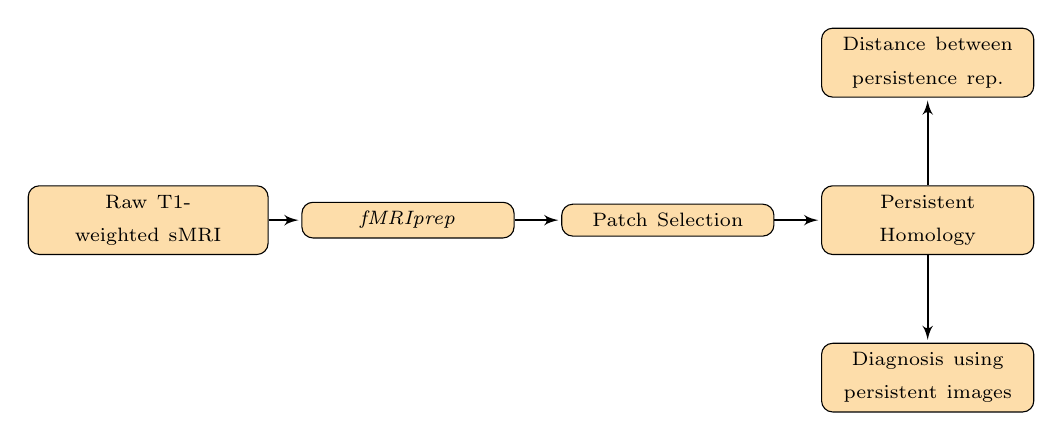
\begin{tikzpicture}[align=center, node distance = 1.8cm, auto]
    \node[orange, text width=8em](raw){\scriptsize Raw T1-weighted sMRI};
    \onslide<2->{
      \node[orange, right of=raw, xshift=1.5cm](fmriprep){\scriptsize \textit{fMRIprep}};
    \draw[myarrow](raw.east)--(fmriprep.west);
  }
  \onslide<3->{
    \node[orange, right of=fmriprep, xshift=1.5cm](patch){\scriptsize Patch Selection};
    \draw[myarrow](fmriprep.east)--(patch.west);}
  \onslide<4->{
    \node[orange, right of=patch, xshift=1.5cm](ph){\scriptsize Persistent Homology};
    \draw[myarrow](patch.east)--(ph.west);}
  \onslide<5->{
    \node[orange, below of=ph, yshift=-0.2cm](diag){\scriptsize Diagnosis using persistent images};
    \draw[myarrow](ph.south)--(diag.north);}
  \onslide<6->{
    \node[orange, above of=ph, yshift=0.2cm](dist){\scriptsize Distance between persistence rep.};
    \draw[myarrow](ph.north)--(dist.south);}
\end{tikzpicture}
\end{center}
\end{frame}


\begin{frame}[fragile]{Analysis setting}
\begin{figure}
  \centering
  \includegraphics[width=0.4\textwidth]{figures/patch_performance.png}
  \caption{AUCPRC on each patch, achieved using a model described in earlier work. Chosen patch for analyses is boxed in red (patch with highest accuracy).}
\end{figure}
\end{frame}

\begin{frame}[fragile]{I - Diagnosis prediction}
  \begin{itemize}
  \onslide<2->\item Computed the cubical filtration to obtain persistence image for each patch
  \onslide<3->\item Simple CNN to classify AD/CN patients.
  \onslide<4->\item Use same partition as NeurIPS submission, train ANN 3 times on each partition
  \end{itemize}
\end{frame}

\begin{frame}[fragile]{I - Persistent homology}
  \minipage{0.32\textwidth}
  \begin{figure}
    \centering
    \includegraphics[width=\textwidth]{figures/PDs/persistence_diagram_CN.png}
    \caption{CN}
  \end{figure}
  \endminipage
  \hfill
  \minipage{0.32\textwidth}
  \begin{figure}
    \centering
    \includegraphics[width=\textwidth]{figures/PDs/persistence_diagram_MCI.png}
    \caption{MCI}
  \end{figure}%
  \endminipage
  \hfill
  \minipage{0.32\textwidth}
  \begin{figure}
    \centering
    \includegraphics[width=\textwidth]{figures/PDs/persistence_diagram_AD.png}
    \caption{AD}
  \end{figure}
  \endminipage
\end{frame}


\begin{frame}[fragile]{I - Diagnosis prediction - Persistence Images}
\begin{figure}
  \centering
  \begin{subfigure}{0.32\textwidth}
    \includegraphics[width=\textwidth]{figures/PIs/Persistence_image_CN_h_0.png}
  \end{subfigure}
  \begin{subfigure}{0.32\textwidth}
    \includegraphics[width=\textwidth]{figures/PIs/Persistence_image_CN_h_1.png}
  \end{subfigure}
    \begin{subfigure}{0.32\textwidth}
    \includegraphics[width=\textwidth]{figures/PIs/Persistence_image_CN_h_2.png}
  \end{subfigure}
  \onslide<2->\begin{subfigure}{0.32\textwidth}
    \includegraphics[width=\textwidth]{figures/PIs/Persistence_image_AD_h_0.png}
  \end{subfigure}
  \begin{subfigure}{0.32\textwidth}
    \includegraphics[width=\textwidth]{figures/PIs/Persistence_image_AD_h_1.png}
  \end{subfigure}
  \begin{subfigure}{0.32\textwidth}
    \includegraphics[width=\textwidth]{figures/PIs/Persistence_image_AD_h_2.png}
  \end{subfigure}
  \caption{Columns: hom. dimension (0,1,2); Row: Diagnostic category (CN top, AD bottom).}
  \label{fig:sample_rep_pi}
\end{figure}

\end{frame}


\begin{frame}[fragile]{I - Diagnosis prediction - Network architecture}
  \begin{figure}
    \centering
    \includegraphics[width=\textwidth]{figures/model.png}
  \end{figure}
\end{frame}


\begin{frame}[fragile]{I - Diagnosis prediction - Performance}
\begin{table}
  \centering
  \begin{tabular}{lc}
    \toprule
    \textbf{Performance metric} & \textbf{Model trained on PIs from patches}\\
    \midrule
    Training accuracy & $0.81\pm 0.01$  \\
    Validation accuracy & $0.78\pm 0.03$  \\
    Precision & $0.81\pm 0.04$  \\
    Recall & $0.77\pm 0.03$  \\
    AUC & $0.85\pm 0.03$  \\
    \bottomrule
    \vspace{1pt}
  \end{tabular}
  \caption{Performance metrics of the model.}
  \label{tab:performance}
\end{table}
\onslide<2->$\rightarrow$ using a normal CPU, training  takes 1 minute!
\end{frame}

\begin{frame}[fragile]{II - Distance analysis among patients in CN, MCI \& AD}
\textbf{Question:} How topologically heterogenous is the data?
  \begin{itemize}
  \onslide<2->\item Compute a persistence landscape (allows for statistical analysis)
  \onslide<3->\item Compute a median persistence landscape with one layer for each category (CN, MCI, AD)
  \onslide<4->\item Compute $L^1$ norm from median landscape for each image within category
  \end{itemize}
\end{frame}


\begin{frame}[fragile]{II - Distance analysis among patients in CN, MCI \& AD}
  Median persistence landscape.\\
  \minipage{0.32\textwidth}
  \begin{figure}
    \centering
    \includegraphics[width=\textwidth]{figures/median_pls/median_pl_CN.png}
    \caption{CN}
  \end{figure}
  \endminipage
  \hfill
  \minipage{0.32\textwidth}
  \begin{figure}
    \centering
    \includegraphics[width=\textwidth]{figures/median_pls/median_pl_MCI.png}
    \caption{MCI}
  \end{figure}%
  \endminipage
  \hfill
  \minipage{0.32\textwidth}
  \begin{figure}
    \centering
    \includegraphics[width=\textwidth]{figures/median_pls/median_pl_AD.png}
    \caption{AD}
  \end{figure}
  \endminipage
\end{frame}

\begin{frame}[fragile]{II - Distance analysis among patients in CN, MCI \& AD}
\textbf{Question:} How topologically heterogenous is the data?
\begin{table}
\centering
\begin{tabular}{lrrrrrr}
\toprule
{} &  Mean &  Median &  Standard deviation &   Q3 &   Max &  Skewness \\
\midrule
CN $H_0$ & 2.16 & 2.00 & 0.78 & 2.50 & 7.41 & 1.78 \\
CN $H_1$ & 2.61 & 2.27 & 1.17 & 2.93 & 9.47 & 1.92 \\
CN $H_2$ & 2.38 & 2.23 & 0.88 & 2.79 & 7.19 & 1.39 \\
MCI $H_0$ & 2.24 & 2.04 & 0.82 & 2.55 & 6.21 & 1.71 \\
MCI $H_1$ & 2.57 & 2.19 & 1.29 & 2.80 & \textbf{11.87} & \textbf{2.57} \\
MCI $H_2$ & 2.40 & 2.27 & 0.83 & 2.82 & 6.55 & 1.18 \\
AD $H_0$ & 2.40 & 2.18 & 0.96 & 2.77 & 7.77 & 1.97 \\
AD $H_1$ & 2.47 & 2.13 & 1.15 & 2.77 & \textbf{9.28} & \textbf{2.10} \\
AD $H_2$ & 2.36 & 2.20 & 0.80 & 2.75 & 8.39 & 1.64 \\
  \bottomrule
\end{tabular}
\caption{Summary statistics of the distribution of distances }
\label{tab:stats_median_pl}
\end{table}
\end{frame}

\begin{frame}[fragile]{III - Distance analysis among patients who deteriorate vs. those who don't}
\textbf{Question:} Among the patients who deteriorate, do we see higher average pairwise distances compared to patients who don't deteriorate?
  \begin{itemize}
  \onslide<2->\item The data is a longitudinal dataset (multiple timepoints are available for each patient)
  \onslide<3->\item Some patients deteriorate (transition from CN$\rightarrow$MCI or from MCI$\rightarrow$AD)
  \onslide<4->\item Compute pairwise distance between patients ($L^1$ PL distance, Wasserstein distance and bottleneck distance), and average for each patient.
  \end{itemize}
\end{frame}

\begin{frame}[fragile]{III - Distance analysis among patients who deteriorate vs. those who don't}
  Example of $L^1$ norm between PLs of a deteriorating patient.\\
  \minipage{0.32\textwidth}
  \begin{figure}
    \centering \includegraphics[width=\textwidth]{figures/temporal_evolution/ADNI029S0878_h_0.png}
    \caption{$H_0$}
  \end{figure}
  \endminipage
  \hfill
  \minipage{0.32\textwidth}
  \begin{figure}
    \centering
    \includegraphics[width=\textwidth]{figures/temporal_evolution/ADNI029S0878_h_1.png}
    \caption{$H_1$}
  \end{figure}%
  \endminipage
  \hfill
  \minipage{0.32\textwidth}
  \begin{figure}
    \centering
    \includegraphics[width=\textwidth]{figures/temporal_evolution/ADNI029S0878_h_2.png}
    \caption{$H_2$}
  \end{figure}
  \endminipage
\end{frame}

\begin{frame}[fragile]{III - Distance analysis among patients who deteriorate vs. those who don't}
  Example of $L^1$ norm between PLs of a subject who does \emph{not} deteriorate.\\
  \minipage{0.32\textwidth}
  \begin{figure}
    \centering
    \includegraphics[width=\textwidth]{figures/temporal_evolution/ADNI011S0023_h_0.png}
    \caption{$H_0$}
  \end{figure}
  \endminipage
  \hfill
  \minipage{0.32\textwidth}
  \begin{figure}
    \centering
    \includegraphics[width=\textwidth]{figures/temporal_evolution/ADNI011S0023_h_1.png}
    \caption{$H_1$}
  \end{figure}%
  \endminipage
  \hfill
  \minipage{0.32\textwidth}
  \begin{figure}
    \centering
     \includegraphics[width=\textwidth]{figures/temporal_evolution/ADNI011S0023_h_2.png}
    \caption{$H_2$}
  \end{figure}
  \endminipage
\end{frame}

\begin{frame}[fragile]{III - Distance analysis among patients who deteriorate vs. those who don't}
Persistence landscape $L^1$ norm\\
  \minipage{0.32\textwidth}
  \begin{figure}
    \centering
    \includegraphics[width=\textwidth]{figures/temporal_evolution/landscape_H_0_dist_diag_change.png}
    \caption{$H_0$}
  \end{figure}
  \endminipage
  \hfill
  \minipage{0.32\textwidth}
  \begin{figure}
    \centering
    \includegraphics[width=\textwidth]{figures/temporal_evolution/landscape_H_1_dist_diag_change.png}
    \caption{$H_1$}
  \end{figure}%
  \endminipage
  \hfill
  \minipage{0.32\textwidth}
  \begin{figure}
    \centering
     \includegraphics[width=\textwidth]{figures/temporal_evolution/landscape_H_2_dist_diag_change.png}
    \caption{$H_2$}
  \end{figure}
  \endminipage
\end{frame}


\begin{frame}[fragile]{III - Distance analysis among patients who deteriorate vs. those who don't}
Bottleneck $L^1$ norm\\
  \minipage{0.32\textwidth}
  \begin{figure}
    \centering
    \includegraphics[width=\textwidth]{figures/temporal_evolution/bottleneck_H_0_dist_diag_change.png}
    \caption{$H_0$}
  \end{figure}
  \endminipage
  \hfill
  \minipage{0.32\textwidth}
  \begin{figure}
    \centering
    \includegraphics[width=\textwidth]{figures/temporal_evolution/bottleneck_H_1_dist_diag_change.png}
    \caption{$H_1$}
  \end{figure}%
  \endminipage
  \hfill
  \minipage{0.32\textwidth}
  \begin{figure}
    \centering
     \includegraphics[width=\textwidth]{figures/temporal_evolution/bottleneck_H_2_dist_diag_change.png}
    \caption{$H_2$}
  \end{figure}
  \endminipage
\end{frame}


\begin{frame}[fragile]{III - Distance analysis among patients who deteriorate vs. those who don't}
Wasserstein distance\\
  \minipage{0.32\textwidth}
  \begin{figure}
    \centering
    \includegraphics[width=\textwidth]{figures/temporal_evolution/wasserstein_H_0_dist_diag_change.png}
    \caption{$H_0$}
  \end{figure}
  \endminipage
  \hfill
  \minipage{0.32\textwidth}
  \begin{figure}
    \centering
    \includegraphics[width=\textwidth]{figures/temporal_evolution/wasserstein_H_1_dist_diag_change.png}
    \caption{$H_1$}
  \end{figure}%
  \endminipage
  \hfill
  \minipage{0.32\textwidth}
  \begin{figure}
    \centering
     \includegraphics[width=\textwidth]{figures/temporal_evolution/wasserstein_H_2_dist_diag_change.png}
     \caption{$H_2$}
  \end{figure}
  \endminipage
\end{frame}

\begin{frame}[fragile]{Limitations \& Outlook}
  \begin{enumerate}
  \item Diagnosis
    \begin{itemize}
    \onslide<2-> \item Performance can be enhanced by taking local features from other patches and passing them through convolutions. Especially useful when dealing with subtypes of Alzheimer's which show atrophy in other brain regions.
    \onslide<3-> \item Neural architecture could be made more complex to capture more complex features of the persistence images
    \onslide<4-> \item Can persistence images be used to diagnose prodromal forms of AD?
  \end{itemize}
  \onslide<5-> \item Distances
    \begin{itemize}
    \onslide<5-> \item In general, very \emph{coarse} analysis (averages do not pick out subtypes or use individual features to differentiate between images), sensitive to noise.
    \onslide<7-> \item Could learn better (topology-based) embeddings to better distinguish between people who progress versus those who do not and more finegrained subtype identification resilient noise.
    \end{itemize}
  \end{enumerate}
\end{frame}


\begin{frame}{Summary}

  GitHub repository of the project

  \begin{center}\url{github.com/pjhartout/TDA_ADNI_MLCB}\end{center}

  With thanks to Bastian Rieck for the   supervision and Sarah Brueningk, Felix Hensel, Catherine Jutzeler, Merel Kuijs and Louis Lukas for insightful discussions, code, and data.

\end{frame}


\begin{frame}[standout]
  Questions?
\end{frame}

% Slides below provided for reference so we don't need to look things up,

% \begin{frame}[fragile]{Context}
%     Predictable geometries arise when \textit{minimising surface energy} or \textit{maximising space filling} in biological and non-biological structures:
%     \begin{columns}[T,onlytextwidth]
%         \column{0.5\textwidth}
%           Examples
%           \begin{itemize}
%             \item \textit{Drosophila Melanogaster}'s retinal cells \item Honeycombs \item Coins on tabletops
%           \end{itemize}

%         \column{0.5\textwidth}
%             \begin{figure}
%                 \centering
%                 \includegraphics[width=.5\textwidth]{figures/honeycombs.png}
%                 \label{}
%             \end{figure}
%     \end{columns}
%     \vspace{12pt}
%     \onslide<2->How is the geometry of \emph{growing} epithelial cells organized and how can it be explained?
% \end{frame}


% \begin{frame}[fragile]{Recurrence system}
%   \begin{columns}
%   \column{0.6\textwidth}
%   \begin{table}
%     \caption{Cell features, topological equivalence and evolution at division $t$}
%     \scalebox{0.9}{
%     \begin{tabular}{lll}
%       \toprule
%       Cell feature & Graph equivalent & Evolution at division $t$\\
%       \midrule
%       Tricellular junction & Vertex, $v_t$ & $v_t=v_{t-1}+2f_t$\\
%       Cell side & Edge, $e_t$ & $e_t=e_{t-1}+3f_{t-1}$\\
%       Apical cell surface & Face, $f_t$ & $e_t=e_{t-1}+3f_{t-1}$\\
%       \bottomrule
%     \end{tabular}
%     }
%   \end{table}
%   \column{0.4\textwidth}
%   So we can construct the following system:
%   \begin{equation*}
%     s_t=\frac{2(e_t+3f_{t-1})}{2f_{t-1}}=\frac{s_{t-1}}{2}+3
%   \end{equation*}
%   which exponentially converges to 6 provided the initial condition:
%   \begin{equation*}
%     s_t=6+2^{-t}(s_0-6)
%   \end{equation*}
% \end{columns}
% \end{frame}

\end{document}